% このバージョンのCVPRテンプレートはMing-Ming Chengによって提供されています。
% バグを見つけた場合は、以下のリンクから問題を報告してください:
% https://github.com/MCG-NKU/CVPR_Template.

%\documentclass[review]{cvpr}
\documentclass[final]{cvpr}
\usepackage[UTF8]{ctex}
\usepackage{enumitem}
\usepackage{times}
\usepackage{epsfig}
\usepackage{graphicx}
\usepackage{amsmath}
\usepackage{amssymb}
\usepackage{makecell}
\usepackage{booktabs}
\usepackage[table,xcdraw]{xcolor}
\usepackage{multirow}
\usepackage{bbm}

% 他のパッケージは、hyperrefの前にここに含めてください。

% hyperrefをコメントアウトしてから再度コメントを外す場合、
% egpaper.auxを削除してからlatexを再実行する必要があります。
% (または、最初のlatex実行時に'q'を押して、完了させるとクリアになります)。
\usepackage[pagebackref=true,breaklinks=true,colorlinks,bookmarks=false]{hyperref}

\def\cvprPaperID{4107} % *** ここにCVPRペーパーIDを入力してください
\def\confYear{CVPR 2021}
%\setcounter{page}{4321} % 最終バージョンのみ

\begin{document}

\title{Railroad is not a Train: Saliency as Pseudo-pixel Supervision \ for Weakly Supervised Semantic Segmentation}

\author{Seungho Lee\thanks{ indicates an equal contribution.}\
Yonsei University\\
{\tt\small seungholee@yonsei.ac.kr}
% すべての著者が同じ機関に所属している場合、
% 以下の行を閉じる"}"まで省略してください。
% 追加の著者と住所は"\and"で追加できます。
% メールアドレスまたはホームページのどちらか一方を使用してスペースを節約してください。
\and
Minhyun Lee\footnotemark[1]\\
Yonsei University\\
{\tt\small lmh315@yonsei.ac.kr}
\and 
Jongwuk Lee\\
Sungkyunkwan University\\
{\tt\small jongwuklee@skku.edu}
\and 
Hyunjung Shim\thanks{Hyunjung Shim is a corresponding author.}\\
Yonsei University\\
{\tt\small kateshim@yonsei.ac.kr}
}

\maketitle
\thispagestyle{empty}
\pagestyle{empty}

%%%%%%%%% ABSTRACT

\begin{abstract}
既存の画像レベルの弱い監視を使用した弱教師ありセマンティックセグメンテーション(WSSS)の研究には、いくつかの制限があります:オブジェクトのカバレッジが疎であること、不正確なオブジェクトの境界、非ターゲットオブジェクトからの共起ピクセル。これらの課題を克服するために、我々は新しいフレームワーク、すなわちExplicit Pseudo-pixel Supervision(EPS)を提案します。これは、ローカライゼーションマップを介してオブジェクトのアイデンティティを提供する画像レベルのラベルと、オフ・ザ・シェルフの顕著性検出モデルからの顕著性マップが豊富な境界を提供することによって、ピクセルレベルのフィードバックから学習します。我々は、両方の情報の補完的な関係を完全に活用するための共同トレーニング戦略を考案しました。我々の方法は、正確なオブジェクトの境界を取得し、共起ピクセルを破棄することができ、擬似マスクの品質を大幅に向上させます。実験結果は、提案された方法がWSSSの主要な課題を解決することにより、既存の方法を著しく上回り、PASCAL VOC 2012およびMS COCO 2014データセットの両方で新しい最先端のパフォーマンスを達成することを示しています。コードは\href{https://github.com/halbielee/EPS}{https://github.com/halbielee/EPS}で利用可能です。
\end{abstract}


\section{Introduction}

弱教師ありセマンティックセグメンテーション(WSSS)は、弱い監視(\eg, 画像レベルのラベル~\cite{pathak2015constrained, pinheiro2015image}, スクリブル~\cite{lin2016scribblesup}, またはバウンディングボックス~\cite{khoreva2017simple})を利用し、ピクセルレベルのラベルを必要とする完全教師ありモデルに匹敵するパフォーマンスを達成することを目指しています。ほとんどの既存の研究は、セグメンテーションモデルの弱い監視として画像レベルのラベルを採用しています。WSSSの全体的なパイプラインは2つのステージで構成されています。まず、画像分類器を使用してターゲットオブジェクトのための擬似マスクが生成されます。次に、セグメンテーションモデルは監視として擬似マスクを使用して訓練されます。擬似マスクを生成するための一般的な技術は、クラスアクティベーションマッピング(CAM)~\cite{zhou2016learning}であり、画像レベルのラベルに対応するオブジェクトのローカライゼーションマップを提供します。完全(\ie, ピクセルレベルのアノテーション)と弱(\ie, 画像レベルのラベル)教師ありセマンティックセグメンテーションの間の監視ギャップのために、WSSSには以下の主要な課題があります:1)ローカライゼーションマップはターゲットオブジェクトのごく一部しかキャプチャしない~\cite{zhou2016learning}、2)オブジェクトの境界の不一致に苦しむ~\cite{kim2017two}、3)ターゲットオブジェクトからの共起ピクセルをほとんど分離できない(\eg, 列車からの鉄道)~\cite{kolesnikov2016seed}。

\begin{figure}[t]
\centering
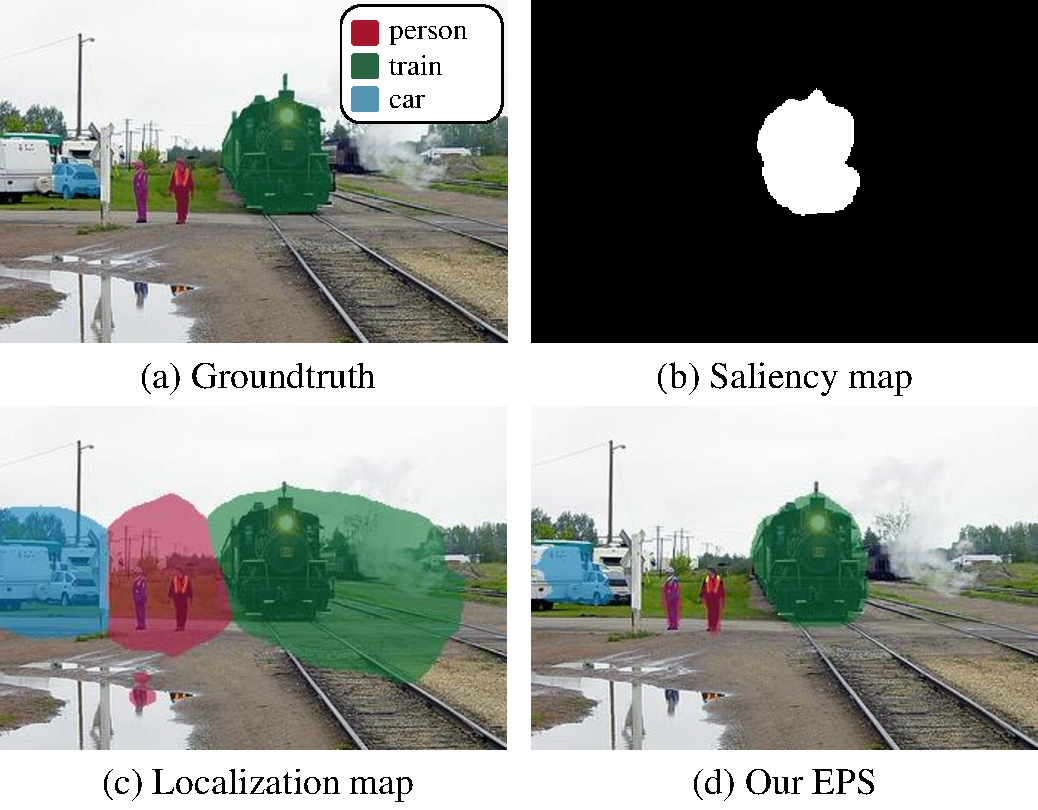
\includegraphics[width=8 cm]{figures/fig_concept.pdf}
\caption{Motivating example of utilizing both the saliency map and the localization map for WSSS. (a) Groundtruth, (b) saliency map via PFAN~\cite{zhao2019pyramid}, (c) localization map via CAM~\cite{zhou2016learning} and (d) our EPS utilizing both the saliency map and the localization map for training a classifier. Note that the saliency map cannot capture \emph{person} and \emph{car} while our result can correctly restore them, and the localization map overly captures two objects.} \vspace{-2mm}
\label{fig:concept}
\end{figure}

これらの問題に対処するために、既存の研究は3つの柱に分類できます。最初のアプローチは、ピクセルを消去することによってオブジェクトの全体を捉えるためにオブジェクトのカバレッジを拡大することです~\cite{choe2020attention,kim2017two, li2018tell}、スコアマップをアンサンブルすること~\cite{jiang2019integral, lee2019ficklenet}、または自己教師あり信号を使用すること~\cite{wang2020self}です。しかし、これらの方法は、オブジェクトの形状を導く手がかりがないため、ターゲットオブジェクトの正確な境界を決定することができません。第二のアプローチは、擬似マスクのオブジェクト境界を改善することに焦点を当てています~\cite{fan2020learning,chen2020boundary}。これらは効果的にオブジェクトの境界を学習するため、自然に擬似マスクを境界まで拡張します。しかし、依然として非ターゲットオブジェクトの重複ピクセルをターゲットオブジェクトから区別することができません。これは、前景と背景の強い相関関係(\ie、共起)が、ターゲットオブジェクトとその重複ピクセルを観察する頻度(\ie、帰納的バイアス)とほとんど区別がつかないためです~\cite{choe2020evaluating}。最後に、第三のアプローチは、追加のグラウンドトゥルースマスク~\cite{BMVC2016_92}や顕著性マップ~\cite{oh2017exploiting, yao2020saliency}を使用して共起問題を軽減することを目的としています。しかし、\cite{BMVC2016_92,li2018tell}は、弱教師あり学習パラダイムからは程遠い強いピクセルレベルのアノテーションを必要とします。\cite{oh2017exploiting}は顕著性マップのエラーに敏感です。また、\cite{yao2020saliency}はオブジェクトの全体をカバーせず、境界の不一致に苦しんでいます。

本論文では、画像レベルのラベルで訓練された画像分類器からのCAM(\ie、ローカライゼーションマップ)と、既製の顕著性検出モデルの出力(\ie、顕著性マップ)を完全に活用することにより、WSSSの3つの課題を克服することを目指します。ローカライゼーションマップと顕著性マップの補完的な関係に焦点を当てます。図~\ref{fig:concept}に示すように、ローカライゼーションマップは異なるオブジェクトを区別できますが、その境界を効果的に分離することはできません。対照的に、顕著性マップは豊富な境界情報を提供しますが、オブジェクトの識別を明らかにしません。この意味で、2つの補完的な情報を使用する我々の方法がWSSSのパフォーマンスボトルネックを解決できると主張します。

この目的のために、我々はWSSSのための新しいフレームワーク、\emph{Explicit Pseudo-pixel Supervision (EPS)}を提案します。顕著性マップ(\ie、前景と背景の両方)を完全に活用するために、$C$ターゲットクラスと背景クラスからなる$C+1$クラスを予測する分類器を設計します。$C$ローカライゼーションマップと背景ローカライゼーションマップを活用して顕著性マップを推定します。次に、顕著性損失は、顕著性マップと我々の推定顕著性マップのピクセル単位の差として定義されます。顕著性損失を導入することにより、モデルはすべてのクラスにわたる擬似ピクセルフィードバックによって監督されることができます。また、マルチラベル分類損失を使用して画像レベルのラベルを予測します。したがって、分類器を顕著性損失とマルチラベル分類損失の両方を最適化するように訓練し、背景と前景ピクセルの予測を相乗的に行います。我々の戦略が顕著性マップ(セクション~\ref{section3.3}と図~\ref{fig:sal})と擬似マスク(セクション~\ref{section:5.1}と図~\ref{fig:ablation})の両方を改善できることがわかります。

顕著性損失が擬似ピクセルフィードバックを通じて境界の不一致を罰するため、我々の方法がオブジェクトの正確な境界を学習することを強制できることを強調します。副産物として、境界までマップを拡張することによってオブジェクト全体を捉えることもできます。顕著性損失が前景(\eg、列車)を背景から分離するのを助けるため、我々の方法は共起ピクセル(\eg、鉄道)を背景クラスに割り当てることができます。実験結果は、我々のEPSがPASCAL VOC 2012とMS COCO 2014データセットで新しい最先端の精度を記録し、顕著なセグメンテーション性能を達成することを示しています。

\section{関連研究}

\noindent\textbf{弱教師ありセマンティックセグメンテーション。}
WSSSの一般的なパイプラインは、分類ネットワークから擬似マスクを生成し、その擬似マスクを監督として使用してセグメンテーションネットワークを訓練することです。画像レベルのラベルにおける境界情報の不足により、多くの既存の手法は不正確な擬似マスクに悩まされています。この問題に対処するために、クロスイメージアフィニティ~\cite{fan2020cian}、知識グラフ~\cite{liu2020leveraging}、およびコントラスト最適化~\cite{sun2020mining, zhang2020splitting}が擬似マスクの品質を向上させるために使用されています。\cite{chang2020weakly}は、分類器がCAMを改善するように強制するために、サブカテゴリを発見する自己監督タスクを提案しています。\cite{ahn2019weakly, ahn2018learning}は、ピクセル間のアフィニティを計算することで境界情報を暗黙的に活用しています。\cite{zhang2020reliability}は、信頼性のあるピクセルレベルのアノテーションを生成し、セグメンテーションマップを生成するためのエンドツーエンドネットワークを設計しています。\cite{huang2018weakly, kolesnikov2016seed}は、境界損失を利用してセグメンテーションネットワークを訓練しています。最近では、\cite{araslanov2020single}が自己監督型のトレーニングスキームを持つ単一のセグメンテーションベースのモデルを使用しています。\cite{fan2020employing}は、複数の不完全な擬似マスクを利用してセグメンテーションネットワークのロバスト性に焦点を当てています。

\begin{figure*}[t]
\centering
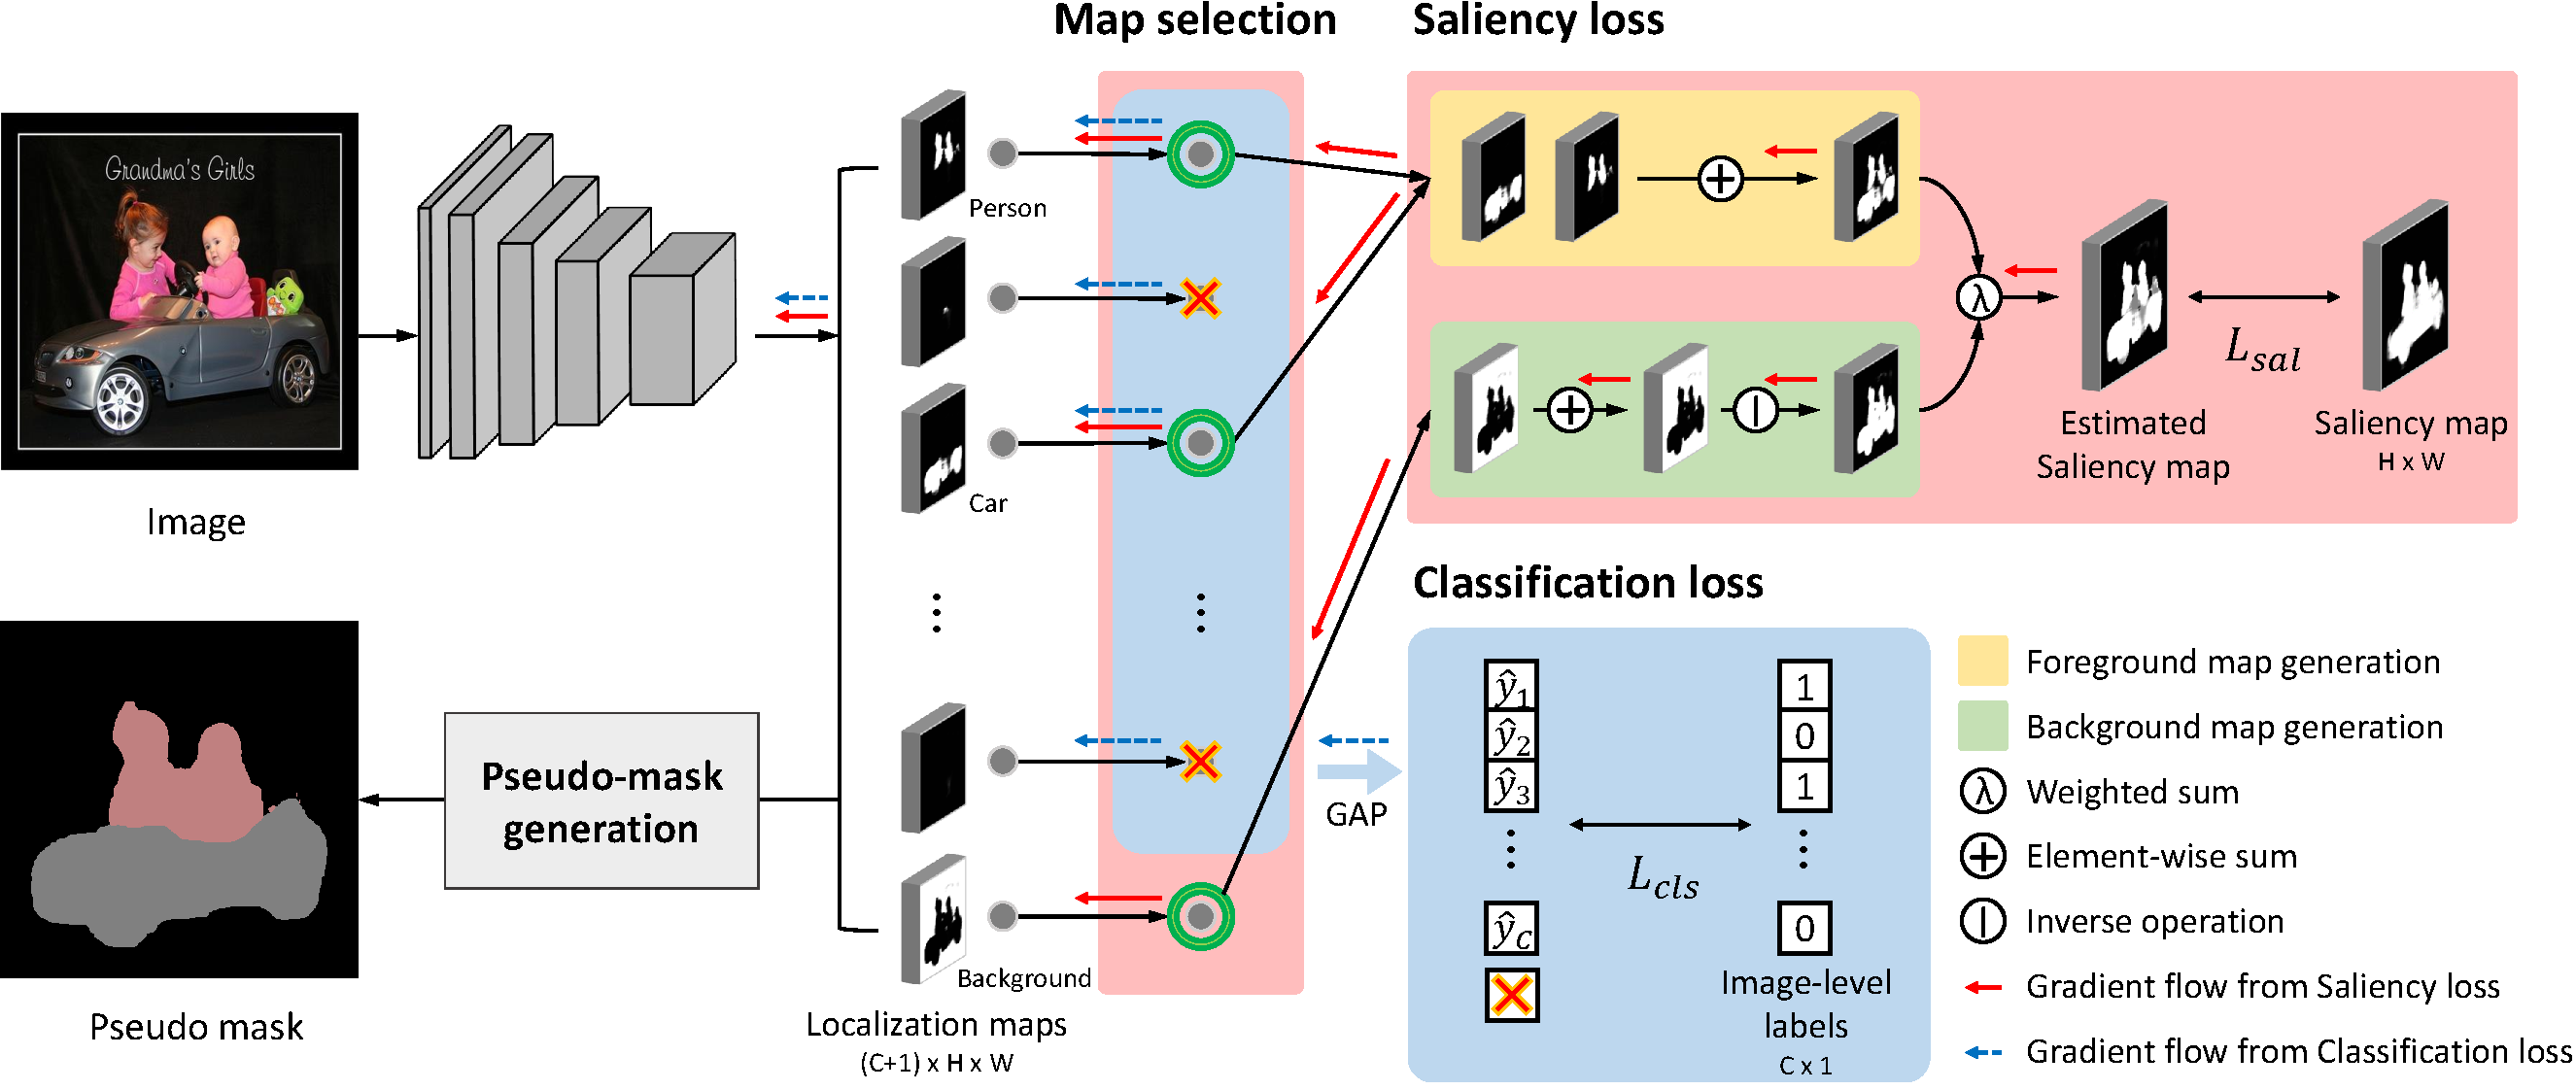
\includegraphics[width=16cm]{figures/framework.pdf}
\caption{我々のEPSの全体的なフレームワーク。$C+1$のローカライゼーションマップがバックボーンネットワークから生成されます。実際の顕著性マップは、既製の顕著性検出モデルから生成されます。ターゲットラベルのためのいくつかのローカライゼーションマップは、推定顕著性マップを生成するために選択的に使用されます(セクション~\ref{section3.2})。全体的なフレームワークは、顕著性損失と分類損失と共に共同で訓練されます(セクション~\ref{section3.3})。} \vspace{-2mm}
\label{fig:framework}
\end{figure*}


\vspace{1mm}
\noindent\textbf{顕著性ガイド付きセマンティックセグメンテーション。}
顕著性検出(SD)手法は、ピクセルレベルのアノテーションを持つ外部の顕著性データセット~\cite{hou2017deeply, xiao2018deep, zhao2019pyramid}、または画像レベルのアノテーション~\cite{wang2017learning}を介して、画像内の前景と背景を区別する顕著性マップを生成します。多くのWSSS手法~\cite{fan2020cian, huang2018weakly, lee2019ficklenet, li2018tell, wei2017object, wei2018revisiting}は、擬似マスクの背景手がかりとして顕著性マップを活用しています。\cite{wei2016stc}は、単一オブジェクト画像の完全な監督として顕著性マップを利用しています。\cite{fan2018associating}は、オブジェクトの類似性グラフを学習するためにインスタンスレベルの顕著性マップを使用しています。\cite{chaudhry_dcsp_2017, wang2018weakly, yao2020saliency}は、クラス固有の注意手がかりと顕著性マップを組み合わせて信頼性のある擬似マスクを生成しています。\cite{zeng2019joint}は、単一のネットワークを使用してWSSSとSDを共同で解決し、両方のタスクのパフォーマンスを向上させています。我々のEPSは顕著性ガイド付き手法に分類されますが、以下の理由で他のすべてと明確に区別されます。既存のほとんどの手法は、擬似マスクの一部として、または分類器の中間特徴を洗練するための暗黙のガイダンスとして顕著性マップを活用しています。対照的に、我々の手法は、ローカリゼーションマップの擬似ピクセルフィードバックとして顕著性マップを利用します。\cite{zeng2019joint}は、2つの補完的な情報を利用するという点で我々の手法に最も類似していますが、共起問題に対処せず、ノイズの多い顕著性マップの問題を扱っていません。

\section{提案手法}

このセクションでは、弱教師ありセマンティックセグメンテーション(WSSS)のための新しいフレームワークである\emph{Explicit Pseudo-pixel Supervision (EPS)}を提案します。WSSSの2つのステージを考慮すると、最初のステージは擬似マスクを生成し、2番目のステージはセグメンテーションモデルを訓練することです。ここでの我々の主な貢献は、正確な擬似マスクを生成することです。WSSSの慣例に従って~\cite{fan2020learning,jiang2019integral,lee2019ficklenet,li2018tell,wang2020self,wei2017object}、最初のステージで生成された擬似マスクを監督として使用してセグメンテーションモデルを訓練します。

\subsection{動機}
\label{section3.1}

EPSの重要な洞察は、ローカリゼーションマップからのオブジェクトアイデンティティと顕著性マップからの境界情報という2つの補完的な情報を完全に活用することです。この目的のために、ターゲットラベルと背景の両方に対して、ローカリゼーションマップへの擬似ピクセルフィードバックとして顕著性マップを利用します。我々は、追加の背景クラスを持つ分類器を考案し、図~\ref{fig:framework}に示すように、合計$C+1$クラスを予測するようにします。この分類器を使用して、ターゲットラベル用の$C$個のローカリゼーションマップと背景ローカリゼーションマップの合計$C+1$個のローカリゼーションマップを学習できます。
次に、EPSがWSSSにおける境界の不一致と共起問題の両方にどのように対処できるかを説明します。境界の不一致問題を管理するために、$C$のローカライゼーションマップから前景マップを推定し、それを顕著性マップの前景と一致させます。この方法により、ターゲットラベルのローカライゼーションマップは顕著性マップから擬似ピクセルフィードバックを受け取り、オブジェクトの境界を改善することができます。非ターゲットオブジェクトの共起ピクセルを軽減するために、背景のローカライゼーションマップも顕著性マップと一致させます。背景のローカライゼーションマップも顕著性マップから擬似ピクセルフィードバックを受け取るため、共起ピクセルは背景にうまく割り当てられます。非ターゲットオブジェクトの共起ピクセルは主に背景と重なっているためです。これが、私たちの方法がターゲットオブジェクトから共起ピクセルを分離できる理由です。
\begin{figure}[t]
\centering
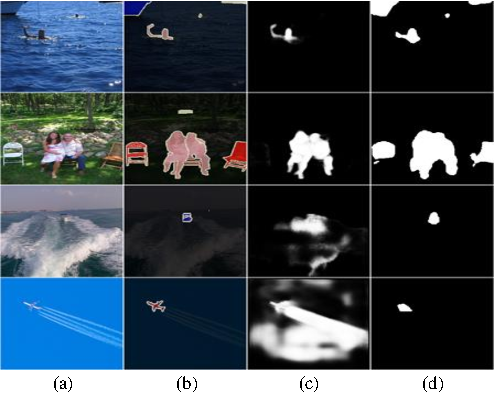
\includegraphics[width=8cm]{figures/fig_saliency_v2.pdf}
\caption{在 PASCAL VOC 2012 上估計的顯著性圖的質性範例。(a) 輸入圖像,(b) 真實值,(c) 來自 \cite{zhao2019pyramid} 的顯著性圖和 (d) 我們估計的顯著性圖。} \vspace{-2mm}
\label{fig:sal}
\end{figure}

最後に、EPSの目的関数は2つの部分で構成されています:顕著性マップを介した{顕著性損失} $\mathcal{L}_{sal}$(図~\ref{fig:framework}の赤いボックス/矢印で示されています)と、画像レベルのラベルを介した{マルチラベル分類損失} $\mathcal{L}_{cls}$(図~\ref{fig:framework}の青いボックス/矢印で示されています)。2つの目的を共同で訓練することにより、ローカライゼーションマップと顕著性マップを補完的な情報でシナジーさせることができます。図~\ref{fig:sal}に示されているように、互いのノイズや欠落情報が私たちの共同訓練戦略を通じて補完されることを観察します。例えば、市販のモデル~\cite{hou2017deeply,nguyen2019deepusps,zhao2019pyramid}から得られた元の顕著性マップには欠落やノイズ情報があります。一方、私たちの結果は欠落したオブジェクト(例:ボートや椅子)をうまく復元し、ノイズ(例:水泡や飛行機雲)を除去し、元の顕著性マップよりも明らかに優れています。その結果、EPSはより正確なオブジェクトの境界をキャプチャし、ターゲットオブジェクトから共起ピクセルを分離することができます。これらの利点は、驚くべき性能向上をもたらします。表~\ref{tab:seg_quan_voc_resnet101}は、EPSが既存のモデルを最大3.8--10.6\%のセグメンテーション精度の向上で著しく上回っていることを報告しています。

\subsection{明示的な擬似ピクセル監督}\label{section3.2}

顕著性マップを擬似ピクセル監督にどのように利用するかを説明します。顕著性マップの主な利点は、オブジェクトのシルエットを提供し、オブジェクトの境界をよりよく明らかにすることです。この特性を利用するために、顕著性マップを前景と背景の2つのケースと一致させます。クラスごとのローカライゼーションマップを顕著性マップと比較可能にするために、ターゲットラベルのローカライゼーションマップをマージし、前景マップ$\mathbf{M}_{fg} \in \mathbb{R}^{H \times W}$を生成します。また、背景ラベルのローカライゼーションマップである背景マップの反転を行うことで前景を表現することもできます(後で、ノイズのある顕著性マップに対処するために前景マップをどのように洗練するかを説明します)。

具体的には、次のようにして$\mathbf{M}_{fg}$と$\mathbf{M}_{bg}$を使用して顕著性マップ$\mathbf{\hat{M}}_{s}$を推定します:\vspace{-1mm}
\begin{equation}
\label{eq_esimate_sal}
{\small
\begin{split}
\mathbf{\hat{M}}_{s} = \lambda\mathbf{M}_{fg} + (1-\lambda)(1-\mathbf{M}_{bg}),
\end{split}}\vspace{-1mm}
\end{equation}
\noindent ここで、$\lambda \in [0, 1]$は前景マップと背景マップの反転の重み付き和を調整するハイパーパラメータです(デフォルトでは、実験で$\lambda$を0.5に設定し、$\lambda$の追加のアブレーション研究は補足資料に記載されています)。次に、推定された顕著性マップと実際の顕著性マップのピクセルごとの差の合計として顕著性損失$\mathcal{L}_{sal}$を定義します($\mathcal{L}_{sal}$の正式な定義はセクション~\ref{section3.3}に示されています)。

事前訓練されたモデルを使用することは弱教師あり学習と見なされるため、顕著性マップを利用することはWSSSで一般的な慣行として広く受け入れられています。その人気にもかかわらず、完全に教師ありの顕著性検出モデルを採用することは、異なるデータセットからのピクセルレベルのアノテーションを使用するため、議論の余地があります。本論文では、異なる顕著性検出方法の効果を調査し、1)教師なしおよび2)完全に教師ありの顕著性検出モデル(セクション~\ref{section5.3}を参照)を使用し、いずれかを使用する私たちの方法が完全に教師ありの顕著性モデルを使用する他のすべての方法~\cite{fan2020learning,jiang2019integral,wang2018weakly, wei2016stc,yao2020saliency}を上回ることを実証的に示します。既存の方法が顕著性マップを完全に活用することに制限されている一方で、私たちの方法は顕著性マップを擬似ピクセル監督として組み込み、境界と共起ピクセルの手がかりとして活用します。

\vspace{1mm}
\noindent\textbf{顕著性バイアスを処理するためのマップ選択。} 以前は、前景マップはターゲットラベルのローカライゼーションマップの合併であり、背景マップは背景ラベルのローカライゼーションマップであると仮定していました。しかし、そのような単純な選択ルールは、市販のモデルによって計算された顕著性マップと互換性がないかもしれません。例えば、\cite{zhao2019pyramid}の顕著性マップは、しばしばいくつかの物体を顕著な物体として無視します(例:図~\ref{fig:concept}の列車の近くにいる小さな人々)。この体系的な誤差は、顕著性モデルが異なるデータセットの統計を学習するため、避けられません。この誤差を考慮しない限り、同じ誤差が我々のモデルに伝播し、性能の低下を引き起こす可能性があります。

この体系的な誤差に対処するために、ローカライゼーションマップと顕著性マップの重なり率を使用した効果的な戦略を開発しました。具体的には、$i$番目のローカライゼーションマップ$\mathbf{M}_{i}$は、顕著性マップと$\tau$\%以上重なっている場合に前景に割り当てられ、それ以外の場合は背景に割り当てられます。形式的には、前景と背景のマップは次のように計算されます:\vspace{-1mm}
\begin{equation}
\label{eq_map_selection}
{\small
\begin{split}
&\mathbf{M}_{fg} = \sum_{i=1}^{C} {y_{i} \cdot \mathbf{M}_{i} \cdot \mathbbm{1}[\mathcal{O}(\mathbf{M}_i, \mathbf{M}_{s}) > \tau]}, \\
&\mathbf{M}_{bg} = \sum_{i=1}^{C} {y_{i} \cdot \mathbf{M}_{i} \cdot \mathbbm{1}[\mathcal{O}(\mathbf{M}_i, \mathbf{M}_{s}) \le \tau]} + \mathbf{M}_{C+1},
\end{split}}\vspace{-1mm}
\end{equation}
\noindent ここで、$y \in \mathbb{R}^C$はバイナリの画像レベルラベルであり、$\mathcal{O}(\mathbf{M}_i, \mathbf{M}_{s})$は$\mathbf{M}_i$と$\mathbf{M}_{s}$の重なり率を計算する関数です。そのために、まずローカライゼーションマップと顕著性マップをバイナライズし、ピクセル$p$に対して、$\mathbf{B}_{k}(p) = 1$ もし$\mathbf{M}_{k}(p) > 0.5$ならば; $\mathbf{B}_{k}(p) = 0$、それ以外の場合。$\mathbf{B}_{i}$と$\mathbf{B}_{s}$はそれぞれ$\mathbf{M}_i$と$\mathbf{M}_{s}$に対応するバイナライズされたマップです。次に、$\mathbf{M}_i$と$\mathbf{M}_{s}$の重なり率を計算します、すなわち、$\mathcal{O}(\mathbf{M}_i ,\mathbf{M}_{s}) = |\mathbf{B}_i \cap \mathbf{B}_{s}| / |\mathbf{B}_{i}|$。データセットやバックボーンモデルに関係なく、$\tau=0.4$に設定します。補足資料では、$\tau$の選択に対して我々の方法が頑健であることを示しています(すなわち、$\tau$が[0.3, 0.5]の範囲であれば、同等の性能を示します)。

背景ラベルの単一のローカライゼーションマップの代わりに、背景ラベルのローカライゼーションマップを前景として選択されなかったローカライゼーションマップと組み合わせます。単純ではありますが、顕著性マップの誤差を回避し、顕著性マップから無視されたいくつかの物体を効果的に訓練することができます。(表~\ref{tab:strategy}では、顕著性マップの誤差を克服するための提案された戦略の有効性を報告しています。)

\subsection{共同訓練手順}\label{section3.3}

顕著性マップと画像レベルのラベルを使用して、EPSの全体的な訓練目標は、顕著性損失$\mathcal{L}_{sal}$と分類損失$\mathcal{L}_{cls}$の2つの部分で構成されています。まず、顕著性損失$\mathcal{L}_{sal}$は、実際の顕著性マップ$\mathbf{M}_{s}$と推定された顕著性マップ$\mathbf{\hat{M}}_{s}$の間の平均ピクセルレベルの距離を測定することによって定式化されます。\vspace{-1mm}
\begin{equation}
{\small
\label{loss_sal}
\mathcal{L}_{sal} = \frac{1}{H\cdot W}||\mathbf{M}_{s}-\mathbf{\hat{M}}_{s}||^{2},
}\vspace{-1mm}
\end{equation}
\noindent ここで、$\mathbf{M}_{s}$はDUTSデータセット~\cite{wang2017learning}で訓練された市販の顕著性検出モデル-- PFAN~\cite{zhao2019pyramid}から取得されます。我々の方法は、顕著性検出モデルに関係なく、すべての以前の技術を一貫して上回ることに注意してください。

次に、分類損失は、画像レベルのラベル$y$とその予測$\hat{y} \in \mathbb{R}^C$の間のマルチラベルソフトマージン損失によって計算されます。これは、各ターゲットクラスのローカライゼーションマップに対するグローバル平均プーリングの結果です。\vspace{-1mm}
\begin{equation}
{\small
\begin{split}
\label{loss_cls}
\mathcal{L}_{cls}= - \frac{1}{C} \sum_{i=1}^{C} y_i \log{\sigma(\hat{y_i})} + (1-y_i) \log{(1 - \sigma(\hat{y_i}))},
\end{split}}\vspace{-1mm}
\end{equation}
\noindent ここで、$\sigma(\cdot)$はシグモイド関数です。最後に、総訓練損失はマルチラベル分類損失と顕著性損失の合計です、すなわち、$\mathcal{L}_{total} = \mathcal{L}_{cls} + \mathcal{L}_{sal}$。
図~\ref{fig:framework}に示すように、$\mathcal{L}_{sal}$は、ターゲットオブジェクトと背景を含む$C+1$クラスのパラメータを更新するのに関与しています。一方、$\mathcal{L}_{cls}$は背景クラスを除く$C$クラスのラベル予測のみを評価し、$\mathcal{L}_{cls}$からの勾配は背景クラスに流れません。しかし、背景クラスの予測は、分類器のトレーニングを監督するため、$\mathcal{L}_{cls}$によって暗黙的に影響を受ける可能性があります。

\section{実験設定}
\noindent
\textbf{データセット}。我々は、PASCAL VOC 2012~\cite{everingham2015pascal}とMS COCO 2014~\cite{lin2014microsoft}という2つの人気のあるベンチマークデータセットで実証研究を行います。PASCAL VOC 2012は21クラス(すなわち、20のオブジェクトと背景)で構成されており、トレーニング、検証、テストセットにはそれぞれ1,464、1,449、1,456枚の画像が含まれています。セマンティックセグメンテーションの一般的な手法に従い、10,582枚の画像を含む拡張トレーニングセットを使用します~\cite{hariharan2011semantic}。次に、COCO 2014は背景を含む81クラスで構成されており、トレーニングと検証にはそれぞれ82,081枚と40,137枚の画像が含まれています。ターゲットクラスがない画像は~\cite{choe2020attention}で行われたように除外されます。一部のオブジェクトのグラウンドトゥルースセグメンテーションラベルが重なっているため、同じCOCOデータセットで重なりの問題を解決するCOCO-Stuff~\cite{caesar2018coco}からのグラウンドトゥルースセグメンテーションラベルを採用します。

\vspace{0.5mm}
\noindent
\textbf{評価プロトコル}。我々の手法をPASCAL VOC 2012の検証セットとテストセット、およびCOCO 2014の検証セットで検証します。PASCAL VOC 2012のテストセットでの評価結果は、公式のPASCAL VOC評価サーバーから取得されます。また、セグメンテーションモデルの精度を測定するために平均交差オーバーユニオン(mIoU)を採用します。

\vspace{0.5mm}
\noindent
\textbf{実装の詳細}。我々の手法のバックボーンネットワークとしてResNet38~\cite{wu2019wider}を選択し、出力ストライドは8です。すべてのバックボーンモデルはImageNet~\cite{deng2009imagenet}で事前トレーニングされています。バッチサイズ8のSGDオプティマイザーを使用します。我々の手法は学習率0.01(最後の畳み込み層は0.1)で20kイテレーションまでトレーニングされます。データ拡張のために、ランダムスケーリング、ランダムフリッピング、およびランダムクロップを$448 \times 448$に使用します。セグメンテーションネットワークには、DeepLab-LargeFOV (V1)~\cite{chen2014semantic}とDeepLab-ASPP (V2)~\cite{chen2017deeplab}、およびそのバックボーンネットワークとしてVGG16とResNet101を採用します。具体的には、VGG16ベースのDeepLab-V1とDeepLab-V2、ResNet101ベースのDeepLab-V1とDeepLab-V2の4つのセグメンテーションネットワークを使用します。詳細な設定は補足資料にあります。

\section{実験結果}

\subsection{境界と共起の処理}\label{section:5.1}

\noindent\textbf{境界不一致問題}。擬似マスクの境界を検証するために、最先端の手法~\cite{chen2020boundary, wang2020self, zhou2016learning}と境界の品質を比較します。PASCAL VOC 2011の境界アノテーションと境界ベンチマークを提供するSBD~\cite{hariharan2011semantic}を利用します。~\cite{chen2020boundary}で行われたように、擬似マスクのエッジをラプラシアンエッジ検出器から計算することにより、クラス非依存の方法で境界の品質を評価します。次に、予測された境界とグラウンドトゥルース境界を比較して、リコール、精度、およびF1スコアを測定することにより、境界の品質を評価します。表~\ref{tab:boundary}は、我々の手法がすべての3つの指標で他の手法を大幅に上回っていることを報告しています。図~\ref{fig:ablation}の定性的な例は、我々の手法が他のすべての手法よりも正確な境界を捉えることができることを示しています。

\begin{figure}[t]
\centering
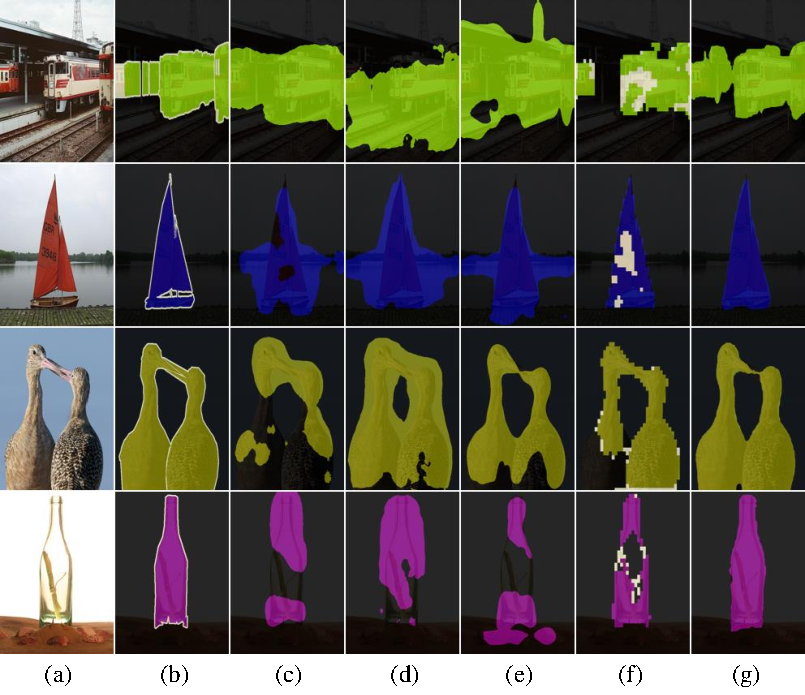
\includegraphics[width=8cm]{figures/fig_ablation.pdf}
\caption{Qualitative comparison for pseudo-masks on PASCAL VOC 2012. (a) Input images, (b) groundtruth, (c) CAM, (d) SEAM, (e) ICD, (f) SGAN and (g) our EPS.}
\label{fig:ablation} \vspace{-3mm}
\end{figure}


\begin{table}[]
\centering
{\small
\begin{tabular}{@{}lccc@{}}
\toprule
\multicolumn{1}{c}{方法}                      & 召回率(\%) & 精确率(\%) & F1-分数(\%) \\ \midrule
\multicolumn{1}{l}{CAM~\cite{zhou2016learning}\textsubscript{CVPR'16}} & 22.3        & 35.8           & 27.5           \\
\multicolumn{1}{l}{SEAM~\cite{wang2020self}\textsubscript{CVPR'20}}    & 40.2        & 45.0           & 42.5           \\
\multicolumn{1}{l}{BES~\cite{chen2020boundary}\textsubscript{ECCV'20}} & 45.5        & 46.4           & 45.9           \\
\multicolumn{1}{l}{我们的 EPS}                        & 60.0        & 73.1          & 65.9           \\ \bottomrule
\end{tabular}
}
\vspace{2mm}
\caption{在 SBD trainval 集上评估的边界准确性。请注意,BES 的结果是从~\cite{chen2020boundary}中提出的边界预测网络测量的。} \vspace{-2mm}
\label{tab:boundary}
\end{table}


\vspace{1mm}
\noindent \textbf{共起問題}。いくつかの研究~\cite{huang2018weakly, kolesnikov2016seed, li2018tell, oh2017exploiting}で議論されているように、PASCAL VOC 2012では、いくつかの背景クラスがターゲットオブジェクトと頻繁に共起することを観察します。PASCAL-CONTEXTデータセット~\cite{mottaghi2014role}を使用して、共起オブジェクトの頻度を定量的に分析します。このデータセットは、シーン全体のピクセルレベルのアノテーションを提供します(例:~\emph{水}と~\emph{鉄道})。3つの共起ペアを選択します;~\emph{ボート}と~\emph{水}、~\emph{列車}と~\emph{鉄道}、および~\emph{列車}と~\emph{プラットフォーム}。ターゲットクラスのIoUとターゲットクラスとその共起クラスの間の~\emph{混同率}を比較します。混同率は、共起クラスがターゲットクラスとして誤って予測される程度を測定します。混同率$m_{k,c}$は、$m_{k,c} = FP_{k,c}/TP_{c}$で計算され、${FP_{k,c}}$は共起クラス$k$のターゲットクラス$c$として誤分類されたピクセル数であり、$TP_{c}$はターゲットクラス$c$の真陽性ピクセル数です。共起問題に関する詳細な分析は補足資料にあります。

Table~\ref{tab:co_quantitative_v4}は、EPSが他の手法よりも一貫して低い混同行列を示すことを報告しています。SGAN~\cite{yao2020saliency}は我々の手法と非常に似た混同行列を持っていますが、我々の手法はIoUの観点でターゲットクラスをより正確に捉えています。興味深いことに、SEAMは高い混同行列を示し、CAMよりも悪い結果を示しています。これは、SEAM~\cite{wang2020self}が自己教師あり学習を適用してターゲットオブジェクトの全範囲をカバーすることを学習するためであり、ターゲットオブジェクトの一致するピクセルに簡単に騙されるからです。一方、CAMはターゲットオブジェクトの最も識別的な領域のみを捉え、あまり識別的でない部分、\eg、一致するクラスをカバーしません。この現象はFigure~\ref{fig:ablation}でも観察できます。

% 請將以下所需的套件添加到您的文件前言:
% \usepackage{booktabs}

\newcommand{\R}{\textcolor{red}}
\newcommand{\B}{\textcolor{blue}}

\begin{table}[]
\centering
{\small
\begin{tabular}{@{}llll@{}}
\toprule
\multicolumn{1}{c}{\multirow{2}{*}{方法}} & \multicolumn{1}{c}{~\emph{船} w/}   & \multicolumn{1}{c}{~\emph{火車} w/}  & \multicolumn{1}{c}{~\emph{火車} w/}  \\
& \multicolumn{1}{c}{~\emph{水}} & \multicolumn{1}{c}{~\emph{鐵路}}          & \multicolumn{1}{c}{~\emph{平台}}  \\ \midrule
\multicolumn{1}{l}{CAM~\cite{zhou2016learning}\textsubscript{CVPR'16}}              & \B{0.74} (33.1)   & \B{0.11} (52.9)   & \multicolumn{1}{l}{\B{0.09} (49.6)}   \\
\multicolumn{1}{l}{SEAM~\cite{wang2020self}\textsubscript{CVPR'20}}                 & \B{1.13} (30.7)   & \B{0.24} (48.6)   & \multicolumn{1}{l}{\B{0.20} (45.5)}   \\
\multicolumn{1}{l}{ICD~\cite{fan2020learning}\textsubscript{CVPR'20}}               & \B{0.47} (41.4)   & \B{0.11} (56.7)   & \multicolumn{1}{l}{\B{0.09} (49.2)}   \\
\multicolumn{1}{l}{SGAN~\cite{yao2020saliency}\textsubscript{ACCESS'20}}            & \B{0.10} (42.3)   & \B{0.02} (48.8)   & \multicolumn{1}{l}{\B{0.01} (36.3)}   \\
\multicolumn{1}{l}{我們的 EPS}                                                         & \B{0.10} (55.0)   & \B{0.02} (78.1)   & \multicolumn{1}{l}{\B{0.01} (73.0)}   \\ \bottomrule
\end{tabular}
}
\vspace{2mm}
\caption{與現有代表性方法處理共現問題的比較。每個條目是 {$m_{k,c}$} 在~\B{藍色}中(越低越好),括號中的 IoU(越高越好)。} \vspace{-2mm}
\label{tab:co_quantitative_v4}

\end{table}

\begin{table}[]
%\resizebox{\columnwidth}{!}{%
\centering

{\small
\begin{tabular}{@{}ccccc@{}}
\toprule
                            & 基线  & 简单   & 预定义   & 我们的自适应 \\ \midrule
\multicolumn{1}{l}{mIoU}    &66.1       & 66.5      & 67.9          & 69.4   \\ \bottomrule
\end{tabular}
}
\vspace{2mm}
\caption{地图选择策略的效果。使用不同地图选择策略的伪掩码的准确性在 PASCAL VOC 2012 训练集上进行评估。} \vspace{-2mm}
\label{tab:strategy}
\end{table}


\subsection{マップ選択戦略の効果}
我々は、サリエンシーマップの誤差を軽減するためのマップ選択戦略の有効性を評価します。我々は、マップ選択モジュールを使用しないベースラインと3つの異なるマップ選択戦略を比較します。単純な戦略として、前景マップはすべてのオブジェクトローカリゼーションマップの和集合であり、背景マップは背景クラスのローカリゼーションマップに等しい(\ie、単純戦略)。次に、以下の例外を除いて単純戦略に従います。いくつかの事前に決定されたクラス(\eg、\emph{ソファ}、\emph{椅子}、\emph{ダイニングテーブル})のローカリゼーションマップは背景マップに割り当てられます(\ie、事前定義クラス戦略)。最後に、提案された選択方法は、ローカリゼーションマップとサリエンシーマップの重なり率を利用し、Section~\ref{section3.2}で説明されているように(\ie、我々の適応戦略)。

\begin{figure*}[t]
\centering
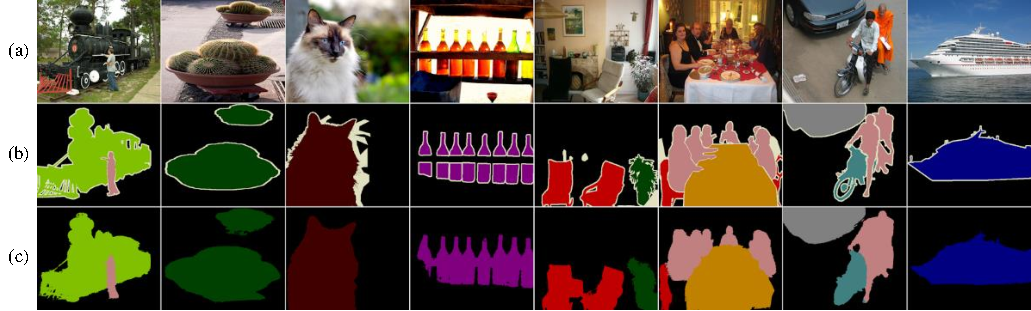
\includegraphics[width=17cm]{figures/segmentation_voc.pdf}
\caption{PASCAL VOC 2012 上分割结果的定性示例。(a) 输入图像,(b) 真实值和 (c) 我们的 EPS。}\vspace{-2mm}
\label{fig:seg_qual_voc}
\end{figure*}

\begin{table}[]
\centering
{\small
\begin{tabular}{@{}lccc@{}}
\toprule
\multicolumn{1}{c}{\multirow{2}{*}{Method}}         & w/o           & w/ &                                  w/ \\
                                                    & refinement    & CRF~\cite{krahenbuhl2011efficient}    & AffinityNet~\cite{ahn2018learning}    \\ \midrule
\multicolumn{1}{l}{CAM~\cite{zhou2016learning}\textsubscript{CVPR'16}}     & 48.0          & -                                     & 58.1                                  \\
\multicolumn{1}{l}{SEAM~\cite{wang2020self}\textsubscript{CVPR'20}}        & 55.4          & 56.8                                  & 63.6                                  \\
\multicolumn{1}{l}{ICD~\cite{chen2020boundary}\textsubscript{CVPR'20}*}     & 59.9          & 62.2                                  & -                                     \\
\multicolumn{1}{l}{SGAN~\cite{yao2020saliency}\textsubscript{ACCESS'20}*}     & 62.8          & -                                     & -                                     \\
\multicolumn{1}{l}{Our EPS}                            & 69.4          & 71.4                                  & 71.6                                  \\ \bottomrule
\end{tabular}
}
\vspace{2mm}
\caption{PASCAL VOC 2012のトレインセットで評価された擬似マスクの精度(mIoU)。*は低信頼度のピクセルが無視されることを示します。他の方法はすべてのピクセルを評価に使用します。} \vspace{-3mm}
\label{tab:refinement}
\end{table}


Table~\ref{tab:strategy}は、我々の適応戦略がサリエンシーマップの体系的なバイアスを効果的に処理できることを示しています。単純戦略は、ローカリゼーションマップから推定されたサリエンシーマップを生成する際にバイアスを考慮しないことを意味します。この場合、擬似マスクの性能は特に\emph{ソファ}、\emph{椅子}、\emph{ダイニングテーブル}クラスで低下します。事前定義クラスを使用することによる性能は、サリエンシーマップで欠落しているクラスを無視することでバイアスを軽減できることを示しています。しかし、人間の観察者による手動選択が必要であるため、実用的ではなく、画像ごとに最適な決定を下すことはできません。一方、我々の適応戦略はバイアスを自動的に処理し、与えられたサリエンシーマップに対してより効果的な決定を下します。

\subsection{最先端技術との比較}
\label{section5.3}

\noindent \textbf{擬似マスクの精度。}我々は、異なるスケールの画像からの予測結果を集約することでマルチスケール推論を採用し、これは~\cite{ahn2018learning,wang2020self}で利用される一般的な手法です。その後、我々は、トレインセットでの擬似マスクの精度を、ベースラインのCAM~\cite{zhou2016learning}および3つの最先端手法、\ie、SEAM~\cite{wang2020self}、ICD~\cite{fan2020learning}、SGAN~\cite{yao2020saliency}と比較して評価します。ここで、トレインセットでの擬似マスクの精度を測定することは、WSSSにおける一般的なプロトコルです。なぜなら、トレインセットの擬似マスクはセグメンテーションモデルを監督するために使用されるからです。Table~\ref{tab:refinement}は擬似マスクの精度を要約し、我々の手法がすべての既存手法を大きな差(\ie、7--21\%のギャップ)で明確に上回っていることを示しています。Figure~\ref{fig:ablation}は擬似マスクの定性的な例を視覚化し、我々の手法がオブジェクトの境界を著しく改善し、擬似マスクの品質において3つの最先端手法を大幅に上回っていることを確認しています。我々の手法はオブジェクトの正確な境界を捉えることができ(2行目)、したがって自然にオブジェクトの全範囲をカバーし(3行目)、一致するピクセルを軽減します(1行目)。我々の手法のさらなる例と失敗例は補足資料で提供されています。

\begin{table}[]
\normalsize
\centering
{\small
\begin{tabular}{@{}lccll@{}}
\toprule
\multicolumn{1}{c}{방법}                                                              & 세그.      & 지원.  & \multicolumn{1}{c}{val} & \multicolumn{1}{c}{test} \\ \midrule
\multicolumn{1}{l}{SEC~\cite{kolesnikov2016seed}\textsubscript{ECCV'16}}                & V1        & I.    & 50.7                    & 51.7                     \\
\multicolumn{1}{l}{AffinityNet~\cite{ahn2018learning}\textsubscript{CVPR'18}}           & V1        & I.    & 58.4                    & 60.5                     \\
\multicolumn{1}{l}{ICD~\cite{fan2020learning}\textsubscript{CVPR'20}}                   & V1        & I.    & 61.2                    & 60.9                     \\
\multicolumn{1}{l}{BES~\cite{chen2020boundary}\textsubscript{ECCV'20}}                  & V1        & I.    & 60.1                    & 61.1                     \\
\multicolumn{1}{l}{GAIN~\cite{li2018tell}\textsubscript{CVPR'18}}                       & V1        & I.+S. & 55.3                    & 56.8                     \\
\multicolumn{1}{l}{MCOF~\cite{wang2018weakly}\textsubscript{CVPR'18}}                   & V1        & I.+S. & 56.2                    & 57.6                     \\
\multicolumn{1}{l}{SSNet~\cite{zeng2019joint}\textsubscript{ICCV'19}}                   & V1        & I.+S. & 57.1                    & 58.6                     \\
\multicolumn{1}{l}{DSRG~\cite{huang2018weakly}\textsubscript{CVPR'18}}                  & V2        & I.+S. & 59.0                    & 60.4                     \\
\multicolumn{1}{l}{SeeNet~\cite{hou2018self}\textsubscript{NeurIPS'18}}                 & V1        & I.+S. & 61.1                    & 60.7                     \\
\multicolumn{1}{l}{MDC~\cite{wei2018revisiting}\textsubscript{CVPR'18}}                 & V1        & I.+S. & 60.4                    & 60.8                     \\
\multicolumn{1}{l}{FickleNet~\cite{lee2019ficklenet}\textsubscript{CVPR'18}}            & V2        & I.+S. & 61.2                    & 61.9                     \\
\multicolumn{1}{l}{OAA~\cite{jiang2019integral}\textsubscript{ICCV'19}}                 & V1        & I.+S. & 63.1                    & 62.8                     \\
\multicolumn{1}{l}{ICD~\cite{fan2020learning}\textsubscript{CVPR'20}}                   & V1        & I.+S. & 64.0                    & 63.9                     \\
\multicolumn{1}{l}{Multi-Est.~\cite{fan2020employing}\textsubscript{ECCV'20}}           & V1        & I.+S. & 64.6                    & 64.2                     \\
\multicolumn{1}{l}{Split. \& Merge.~\cite{zhang2020splitting}\textsubscript{ECCV'20}}   & V2        & I.+S. & 63.7                    & 64.5                     \\
\multicolumn{1}{l}{SGAN~\cite{yao2020saliency}\textsubscript{ACCESS'20}}                & V2        & I.+S. & 64.2                    & 65.0                     \\ \midrule
\multicolumn{1}{l}{\multirow{2}{*}{우리의 EPS}}                                            & V1        & I.+S. & 66.6                    & \textbf{67.9}            \\
\multicolumn{1}{l}{}                                                                    & V2        & I.+S. & \textbf{67.0}           & 67.3                     \\ \bottomrule

\end{tabular}
}
\vspace{2mm}
\caption{PASCAL VOC 2012에서의 세그멘테이션 결과 (mIoU). 모든 결과는 VGG16을 기반으로 합니다. 모든 실험에서 최고의 점수는 굵게 표시되어 있습니다.}\vspace{-3mm}
\label{tab:seg_quan_voc_vgg16}
\end{table}

\begin{table}[]
\normalsize
\centering
{\small
\begin{tabular}{@{}lccll@{}}
\toprule
\multicolumn{1}{c}{Method}                                                              & Seg.      & Sup.  & \multicolumn{1}{c}{val} & \multicolumn{1}{c}{test} \\ \midrule
\multicolumn{1}{l}{ICD~\cite{fan2020learning}\textsubscript{CVPR'20}}                   & V1        & I.    & 64.1                    & 64.3                     \\ 
\multicolumn{1}{l}{SC-CAM~\cite{chang2020weakly}\textsubscript{CVPR'20}}                & V1        & I.    & 66.1                    & 65.9                     \\
\multicolumn{1}{l}{BES~\cite{chen2020boundary}\textsubscript{ECCV'20}}                  & V2        & I.    & 65.7                    & 66.6                     \\
\multicolumn{1}{l}{LIID~\cite{liu2020leveraging}\textsubscript{TPAMI'20}}                  & V2        & I.    & 66.5                    & 67.5                     \\
\multicolumn{1}{l}{MCOF~\cite{wang2018weakly}\textsubscript{CVPR'18}}                   & V1        & I.+S. & 60.3                    & 61.2                     \\
\multicolumn{1}{l}{SeeNet~\cite{hou2018self}\textsubscript{NeurIPS'18}}                 & V1        & I.+S. & 63.1                    & 62.8                     \\
\multicolumn{1}{l}{DSRG~\cite{huang2018weakly}\textsubscript{CVPR'18}}                  & V2        & I.+S. & 61.4                    & 63.2                     \\
\multicolumn{1}{l}{FickleNet~\cite{lee2019ficklenet}\textsubscript{CVPR'18}}            & V2        & I.+S. & 64.9                    & 65.3                     \\
\multicolumn{1}{l}{OAA~\cite{jiang2019integral}\textsubscript{ICCV'19}}                 & V1        & I.+S. & 65.2                    & 66.4                     \\
\multicolumn{1}{l}{Multi-Est.~\cite{fan2020employing}\textsubscript{ECCV'19}}           & V1        & I.+S. & 67.2                    & 66.7                     \\
\multicolumn{1}{l}{MCIS~\cite{sun2020mining}\textsubscript{ECCV'20}}                    & V1        & I.+S. & 66.2                    & 66.9                     \\
\multicolumn{1}{l}{SGAN~\cite{yao2020saliency}\textsubscript{ACCESS'20}}                & V2        & I.+S. & 67.1                    & 67.2                     \\
\multicolumn{1}{l}{ICD~\cite{fan2020learning}\textsubscript{CVPR'20}}                   & V1        & I.+S. & 67.8                    & 68.0                     \\ \midrule
\multicolumn{1}{l}{\multirow{2}{*}{Our EPS}}                                            & V1        & I.+S. & \textbf{71.0}           & \textbf{71.8}            \\
\multicolumn{1}{l}{}                                                                    & V2        & I.+S. & 70.9                    & 70.8                     \\ \bottomrule
\end{tabular}
}
\vspace{2mm}
\caption{PASCAL VOC 2012에서의 세그멘테이션 결과 (mIoU). 모든 결과는 ResNet101을 기반으로 합니다.}\vspace{-2mm}
\label{tab:seg_quan_voc_resnet101}
\end{table}

\begin{figure*}[t]
\centering
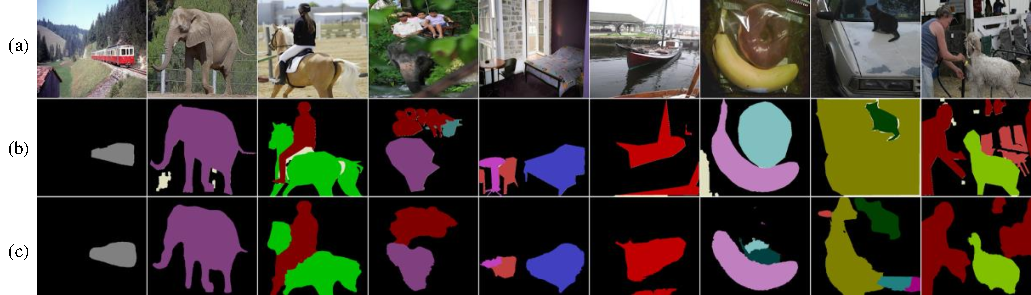
\includegraphics[width=17cm]{figures/segmentation_coco.pdf}
\caption{MS COCO 2014에서의 세분화 결과에 대한 정성적 예시입니다. (a) 입력 이미지, (b) 정답 및 (c) 우리의 EPS.}\vspace{-2mm}
\label{fig:seg_qual_coco} 
\end{figure*}


\vspace{1mm}
\noindent \textbf{セグメンテーションマップの精度。}以前の手法~\cite{ahn2018learning, fan2020learning, wang2020self}は擬似マスクを生成し、CRF後処理アルゴリズム~\cite{krahenbuhl2011efficient}またはアフィニティネットワーク~\cite{ahn2018learning}でそれらを洗練します。一方、Table~\ref{tab:refinement}に示されているように、我々が生成した擬似マスクは十分に正確であるため、擬似マスクの追加の洗練なしにセグメンテーションネットワークを訓練します。我々は、Pascal VOC 2012データセットの4つのセグメンテーションネットワークで我々の手法を他の手法と広範に評価し、正確に比較します。

% Please add the following required packages to your document preamble:
% \usepackage{booktabs}
\begin{table}[]
\centering
{\small
\begin{tabular}{@{}lccc@{}}
\toprule
\multicolumn{1}{c}{Method}                                                  &Seg.       &Sup.   & \multicolumn{1}{c}{val}           \\ \midrule
\multicolumn{1}{l}{SEC~\cite{kolesnikov2016seed}\textsubscript{ECCV'16}}    & V1        &I.     & \multicolumn{1}{c}{22.4}          \\
\multicolumn{1}{l}{DSRG~\cite{huang2018weakly}\textsubscript{CVPR'18}}      & V2        &I.+S.  & \multicolumn{1}{c}{26.0}          \\
\multicolumn{1}{l}{ADL~\cite{choe2020attention}\textsubscript{TPAMI'20}}    & V1        &I.+S.  & \multicolumn{1}{c}{30.8}          \\
\multicolumn{1}{l}{SGAN~\cite{yao2020saliency}\textsubscript{ACESS'20}}     & V2        &I.+S.  & \multicolumn{1}{c}{33.6}          \\ \midrule
\multicolumn{1}{l}{Our EPS}                                                 & V2        &I.+S.  & \multicolumn{1}{c}{\textbf{35.7}} \\ \bottomrule
\end{tabular}
}
\vspace{2mm}
\caption{Segmentation results (mIoU) on MS COCO 2014. All results are based on VGG16.}\vspace{-2mm}
\label{tab:seg_quantitative_coco}
\end{table}

私たちの手法は、セグメンテーションネットワークに関係なく、他の手法よりも著しく優れた性能を発揮します。表~\ref{tab:seg_quan_voc_vgg16}は、同じVGG16バックボーンを使用した場合、私たちの手法が他の手法よりも正確であることを報告しています。さらに、VGG16での私たちの結果は、より強力なバックボーン(\ie 表~\ref{tab:seg_quan_voc_resnet101}のResNet101)に基づく他の既存の手法と比較しても同等かそれ以上です。私たちの手法は、既存の手法に対して明確な改善を示しています。最後に、表~\ref{tab:seg_quan_voc_resnet101}は、ResNet101ベースのDeepLab-V1とサリエンシーマップを使用した私たちの手法が、PASCAL VOC 2012データセットで新しい最先端の性能(検証セットで71.0、テストセットで71.8)を達成したことを示しています。既存の最先端モデルによって達成された向上は約1\%でしたが、私たちの手法は前回の最高記録よりも3\%以上の向上を達成しています。図~\ref{fig:seg_qual_voc}は、PASCAL VOC 2012での私たちのセグメンテーション結果の定性的な例を視覚化しています。これらの結果は、私たちの手法が正確な境界を提供し、共起問題を成功裏に解決することを確認しています。

表~\ref{tab:seg_quantitative_coco}では、COCO 2014データセットで私たちの手法をさらに評価しています。VGG16ベースのDeepLab-V2をセグメンテーションネットワークとして使用し、COCOデータセットでの最先端のWSSSモデルであるSGAN~\cite{yao2020saliency}と比較します。私たちの手法は、検証セットで35.7 mIoUを達成し、SGAN~\cite{yao2020saliency}よりも1.9\%高いです。結果として、COCO 2014データセットで新しい最先端の精度を達成しました。両方のデータセットでの既存の最先端を超えるこれらの優れた性能は、私たちの手法の有効性を確認しています。ローカライゼーションマップとサリエンシーマップの両方を完全に活用することで、ターゲットオブジェクトの全体を正確に捉え、既存モデルの欠点を補います。図~\ref{fig:seg_qual_coco}は、COCO 2014データセットでのセグメンテーション結果の定性的な例を示しています。私たちの手法は、いくつかのオブジェクトが遮蔽されずに現れる場合にうまく機能しますが、多くの小さなオブジェクトを扱うのには効果が低いです。私たちの手法のさらなる例と失敗例は、補足資料で提供されています。

\vspace{1mm}
\noindent \textbf{サリエンシー検出モデルの効果}。異なるサリエンシー検出モデルの効果を調査するために、3つのサリエンシーモデルを採用しました。PFAN~\cite{zhao2019pyramid}(私たちのデフォルト)、OAA~\cite{jiang2019integral}とICD~\cite{fan2020learning}で使用されるDSS~\cite{hou2017deeply}、およびUSPS~\cite{nguyen2019deepusps}(\ie、教師なし検出モデル)です。Resnet101ベースのDeepLab-V1でのセグメンテーション結果(mIoU)は、PFANで71.0/71.8、DSSで70.0/70.1、USPSで68.8/69.9(検証セットとテストセット)です。これらのスコアは、3つの異なるサリエンシーモデルのいずれかを使用しても、私たちのEPSが表~\ref{tab:seg_quan_voc_resnet101}の他のすべての手法よりも正確であることを支持しています。特に、教師なしサリエンシーモデルを使用した私たちのEPSは、教師ありサリエンシーモデルを使用した既存のすべての手法を上回っています。

\section{結論}
私たちは、新しい弱教師ありセグメンテーションフレームワーク、すなわち\emph{明示的擬似ピクセル監督(EPS)}を提案します。ローカライゼーションマップとサリエンシーマップの補完的な関係に動機付けられ、私たちのEPSは、サリエンシーマップとローカライゼーションマップを組み合わせた擬似ピクセルフィードバックから学習します。私たちの共同トレーニングスキームのおかげで、両側のノイズや欠落情報をうまく補完します。その結果、私たちのEPSは正確なオブジェクト境界を捉え、非ターゲットオブジェクトの共起ピクセルを排除し、擬似マスクの品質を著しく向上させます。広範な評価とさまざまなケーススタディは、私たちのEPSの有効性と、PASCAL VOC 2012およびMS COCO 2014データセットの両方でのWSSSの新しい最先端精度を示しています。

\noindent\textbf{謝辞。}
Duhyeon BangとJunsuk Choeにフィードバックを感謝します。この研究は、MSIP(NRF-2019R1A2C2006123、2020R1A4A1016619)によって資金提供されたNRF韓国を通じた基礎科学研究プログラム、MSIT(2020-0-01361、人工知能大学院プログラム(YONSEI UNIVERSITY))によって資金提供されたIITP助成金、および韓国政府によって資金提供された韓国医療機器開発基金助成金(プロジェクト番号:202011D06)によって支援されました。

{\small
\bibliographystyle{ieee_fullname}
\bibliography{egbib}
}

\end{document}
